\section{Scalability Testing}

Currently, on the internet, we have high variation of demand of the applications that run upon it. Many of these applications can not support it properly because of bad implementations or bad architectures. These problems are related to the application scalability. Scalability testing aims at analyzing it and verifying which part of the systems are not scaling properly. Firstly, we need to define what is scalability. Then, we must know how we analyze the application scalability to test it. 

\subsection{Definition of Scalability}
A choreography, in a large scale environment, must be able to attend different scenario sizes. Suppose that a specific choreography, for example, usually receives $N$ requests per second but, in some specific times, receives $10N$ requests per second. It must tolerate this increase of access quickly.

To support this issue, we may increase its system capability between this period of high demand. We want to have the same performance that we had previously. Therefore, we must know how much of resources we should increase to achieve this goal.  Each choreography will have its particular solution. This will depends on how the choreography is implemented. Bad choreographies architectures will need to increase heavily to achieve that, someones won't even achieve.

For instance, in the example above, we could increase the resources in the same scale that the number of access increased to gain the same performance. However, only that will not assure we will perform that, i.e.  the choreography may have a bottleneck that will not disappear if we add more resources. Thus, we also must pay attention in the implementation of the choreography. We gain scalability with the collaboration of the hardware and the software. 

An application is scalable if it achieves the same performance by increasing the architecture capability with the same proportion of the problem size increase. [\citet{QUINN}]. For \citet{LAW}, an application is scalable if the improvements in the execution capability express in direct proportion improvements in architectural capability. However, these definitions just say if an application is scalable or not. Consequently, we can not compare the scalability of two applications by saying that one is more scalable than the other. To conclude how scalable an application is, we need to quantify it. Law quantify simulation scalability in a mathematical model, based on two capabilities, execution and architectural. 

\subsection{Quantifying Scalability}
\label{quantifyingScalability}

The function that quantify the execution capability is based on two functions: the complexity size of the problem function, and the performance metric function. 

The complexity size of the problem is based on a set of values that describe its state, which are called measures of interest. For instance, in a web service stress simulation, the number of requests per second is a measure of interest. If the number of requests per second increases, the complexity size of the problem increases too. The author define the complexity size with the function $S(n_{1}..n_{s})$, where $n_{1}$ to $n_{s}$ is a set of $s$ variables. This variables are the measures of interested. Its assumed that if one of this variables increase, the simulation size function will increase or at least stay the same, but never decrease. There are different ways to define the complexity of a problem. It depends on the characteristics we want to analyze.

%A simulation is built on a set of values that describe its state, this is called measures of interest.  For instance, in a web service stress simulation, the number of requests per second is a measure of interest. If the simulation do not have a minimum satisfactory response time average with correct responses, it did not achieve acceptable performance. 
%We also know it must meet a set of performance requirements. A simulation attain acceptable performance if it execute with correctness and satisfy the performance requirement. , and a performance requirement is the average response time
% Based on the measures of interested and the performance requirements, we can tell the complexity of the problem. 

%We've seen performance as a requirement, however we may also be interested in its precise values. For example, the memory usage may be a metric that we want to minimize even if we have not defined what is the maximum value that it can achieve. 

When we execute the application, a set of performance characteristics can be analyzed. Thus, we also have a function that defines the importance of the metric performances, $M(m_{1}..m_{q})$, where $m_{1}$ to $m_{q}$ is a set of $q$ performance metrics. If a performance metric increases, its assumed that the performance improves. We can reverse the metrics that do not behave this way. If $Y$ is the memory usage metric, we can pass $\frac{1}{Y}$ as input. With these definition we conclude that a simulation capability is the relation of the functions $S$ and $M$, defined as $C(S,M) = S \times M$.

As said previously, to measure scalability we need also to quantify the architectural capability. The inputs that we need to define it are the architecture characteristics, such as the CPU clock speed. The function $P(h_{1}..h_{p})$ describes it, where $h_{1}$ to $h_{p}$ are the variables that represent the measures of the architecture.

With the definition of these two functions, we choose an initial architecture with capability $P_{1}$, initial measures of interested $S_{1}$, and the metric performances $M_{1}$ we want to analyze. After the execution, a constant $k = \frac{C_{1}(S_{1},M_{1})}{P_{1}}$ is calculated. Let $C_{i}$ and $P_{i}$ be capabilities $i$ times greater than $C_{1}$ and $P_{1}$, respectively. Therefore, the author defines scalability as the largest real-value $j$ such as $\frac{C_{i}(S_{i},M_{i})}{P_{i}} \geq k$ for every $i$ in the real-value interval $[1,j]$ and $P_{i}$ can compute $C_{i}(S,M)$ with correctness. With these definition we can are verify the interval where the ratio between the execution capability and the architectural capability stays at least equal as it was initially. If $j = \infty$, we say that the system is fully scalable.

This definition, however, has some limitations as pointed out by Law. One of them is  difficulty to define an architectural capability function that express the exact importance between each hardware characteristic. For example, a system with 512MB of RAM and 100GHz of CPU may have the same capability than one with 256MB and 200GHz of CPU. Another one is about the highly dependency on the definition of the architectural and simulation capabilities in the scalability function. This means that, the same system can have different ranges of scalability depending on how we define these functions. The point here is that is very difficult to quantify the variables P and C. Therefore, if we can not quantify properly them, we won't be able to quantify the scalability of a system. 

These restrictions show us that scalability is something relative, a system may have different ranges of scalability depending on the importance that we gave to its elements. However, despite this limitations, we can adapt it to something more usable. We can use the scalability function to compare two systems with the same architectural and simulation capabilities. We, also, limit the number of the capability functions input to one. Let $s$ be the input of the complexity size of the problem, and $m$ be the input of the performance metric for simulation capability function $C_{i}$ and, $h$ for the architectural capability function. Thus, we can conclude if a system is more scalable then another based on these three variables. Law, presents the final definition of scalability as the largest real-value $j$ such that $\frac{C_{i}(s, m)}{P_{i}(h)} \geq k$ for every i in the real-value interval $[1.0, j]$ and $P_{i}(h)$ can compute $C_{i}(S_{i}(s), M_{i}(m))$ with correctness.

With these description, the author narrow the scalability comparison of two system relative to a specific aspect of the simulation and architectural. For example, we choose $s$ as the size of data send per request to a web service, m as the percentage of used memory, and h as the RAM of the web service hardware. Then we can compare if one system has more scalability than the other in terms of space usage.

\subsection{Quantifying Scalability in Practice}

The definition above, made us conclude that the function $\frac{C_{i}(S_{i},M_{i})}{P_{i}} = \frac{S_{i} \times M_{i}}{P_{i}}$ should be constant after each execution. Therefore, $S_{i} \times M_{i}$ should vary in the same proportion as $P_{i}$. Since the execution capability is based on two functions, $S$ as the complexity size of the problem and $M$ as the performance metric, we can increase it in different ways:
\begin{itemize}
\item Increase S with the same proportion as the architecture capability. In this case, we expect the M to be constant.
\item Fix S. Then, we is expect that M will increase with the same proportion as the architecture capability.
\item Increase S in a different proportion of the architecture capability. Then, we expect that M will increase in a proportion that will make the function $S \times M$ increase with the same proportion as the architecture capability.
\end{itemize}

If we use the first option, the performance metric of an application that has a good scalability should stay constant and one that has a bad scalability will increase. Thus, an application with good scalability will have a performance metric graph with a horizontal line (Figure \ref{fig:goodscalability}) and an application with bad scalability will have an increasing line (Figure \ref{fig:badscalability}).

\begin{figure}[ht]
\begin{minipage}[b]{0.5\linewidth}
\centering
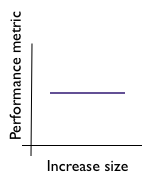
\includegraphics[scale=0.7]{images/scalabilitygood}
\caption{Performance metric graph with \\* a \textbf{good scalability}}
\label{fig:goodscalability}
\end{minipage}
\hspace{0.5cm}
\begin{minipage}[b]{0.5\linewidth}
\centering
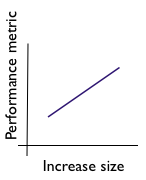
\includegraphics[scale=0.7]{images/scalabilitybad}
\caption{Performance metric graph with \\* a \textbf{bad scalability}}
\label{fig:badscalability}
\end{minipage}
\end{figure}


In this project, we will use the first option because we have control of the variables that define the complexity of the problem and it is easier to visualize in a performance metric graph the difference between an application with good scalability and bad scalability.

\subsection{Types of Scalability}
With the definition presented in the Sub-Section \ref{quantifyingScalability}, we conclude that are different ways to examine the scalability of a system. \cite{BONDI} presents four types of scalability that we can observe:

\begin{description}
\item[Load scalability] A system has more load scalability if it behaves properly with light, moderate or heavy loads. In this case, the word \emph{properly} is related to functional and non-functional aspects, such as resource contention, excessive of delay, and ineffective memory consumption. Thus, to measure the load scalability of a system using the scalability function, we would use, for instance,  number of request per second as the input for the simulation capability function, the number o processor as the input for the architectural capability, and fixing the response time average as a performance metric.
\item[Space scalability]  A system has a bad space scalability if its memory requirements grows largely when the number of supported items increase. For example, measuring the scalability based on the data size sent per request as an input for the simulation capability function, the RAM of the system hardware, and fixing the percentage of RAM used as a performance metric.
\item[Space-time scalability] A system has more space-time scalability if it function properly, without much delays, when the number of its objects increase. If a search system takes more time to find an information because of the increasing of data storage, even if its hardware resources has grown too, we conclude that it does not have space-time scalability.
\item[Structural scalability] A system is structural scalable if it does not prevents the increasing of objects that it encompasses. For example, if a peer-to-peer system has a maximum number of nodes that it support and another has not, then the latter is more structural scalable than the former.
\end{description}

These types of scalability gives us a direction of what we need to observe when comparing the scalability of the systems. Its important to note that they are, sometimes, dependent from each other. A system that needs space-time scalability may also needs space scalability because the huge grown of memory might cause a delay to find information.

\subsection{Related Works}

\cite{STAS} present the Scalability Testing and Analysis System (STAS), a tool that supports the users for running scalability analysis of algorithms and system. STAS analysis scalability using the metric \emph{isospeed-efficiency scalability}, also known as \emph{isospeed-e}. 

The architecture capability used in this metric is the sum of the supported speeds of all system nodes. Let $h_{i}$ be the supported speed of a specific node $i$, then the architecture capability of the system is $P(n) = \sum_{i=1}^{n} h_i$ , where $n$ is the number of nodes. 

A function that characterize the complexity of the problem, defined by the user, combined with the execution time, which is the performance metric, results the simulation capability function $C = \frac{S}{T}$, where $S$ is the value that represents the complexity of the problem and $T$ is the execution time metric. Therefore the scalability function is defined as $\frac{C}{P}$.

STAS is composed by four components as shown in Figure \ref{stasarchitecture}: system characterization component, algorithm pre-analysis component, scalability tester component, and scalability analyzer component.

\begin{figure}[htbp]
\begin{center}
	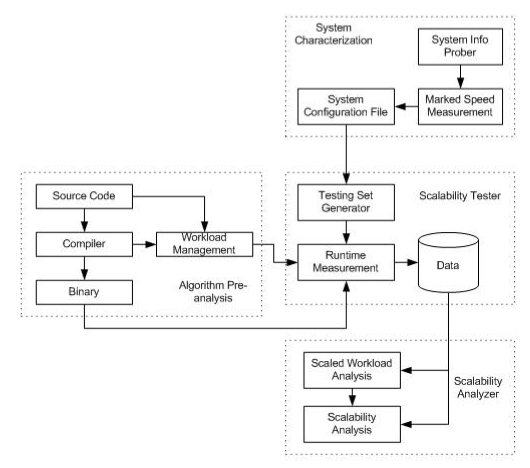
\includegraphics[scale=0.6]{images/stasarchitecture}
\caption{STAS Architecture [\cite{STAS}]}
\label{stasarchitecture}
\end{center}
\end{figure}

The system characterization component is responsible for calculating the supported speed of each node available by measuring their FLOPS. The algorithm pre-analysis component is responsible for calculating the problem complexity defined by the user. 

The scalability tester component executes the application and calculates the execution time.  It calculates $C_1$ by applying the function described above with the values obtained. After that, it execute the application doubling the number of nodes and the parameter of the complexity problem function. $C_2$ is obtained with the execution information. This process is done until it reaches the maximum number of nodes available. The results are compared by the scalability analyzer component that concludes how scalable the application is.

STAS is a scalability testing tool that support only parallel applications, such as MPI, PVM, and HPF. Thus, it is not applicable for SOA applications where the implementation of the services that integrate the system are heterogeneous. It restrict the choice of the scalability function variables. The tester, for instance, cannot test the scalaiblity based on the number of requests per second, since the complexity of the problem is only defined based on the complexity of the application algorithm. The Scalability Testing Framework, described at the next section, aims at providing the freedom to choose the scalability test type desired.

\cite{p2p} presents a methodology and a framework for testing peer-to-peer (P2P) application. The authors combine functional and non-functional tests because in P2P applications volatile and scale changes may happen and might affect the functionalities of the system. The framework is able to manipulate all nodes of the application and tests different scenarios. They apply scalability testing by changing the scales of the application and validating their functionalities. However, each execution scenario must be specified which can make the test specification cumbersome.

Using Java Annotations, the developer specify the behavior and the tests of the nodes. These annotations give to de developer the freedom to manipulate and test the application in different scenarios and scales.










